\documentclass[11pt]{article}
\usepackage[margin=1.5in]{geometry}
\usepackage{fontspec} % Advanced font selection
\setmonofont[Scale=MatchLowercase]{Inconsolatazi4}
\usepackage{amsfonts, amsmath, amssymb, amsthm} % AMS Math Packages
\usepackage{mathtools} % Mathematical tools for amsmath
\usepackage{array, booktabs} % Extends the array and tabular environments
\usepackage{environ} % Interface for environments
\usepackage{parskip, setspace} % Paragraph indentation and line spacing
\usepackage{color} % Color control
\usepackage{colortbl} % Color to tables
\usepackage[x11names]{xcolor} % Color extensions 
\usepackage{soul} % Letter spacing, underlining, striking out 
\usepackage{hyperref} % Support for hypertext
\hypersetup{pdfborder=0 0 0, citebordercolor=Gray0, urlbordercolor=Gray0, linkbordercolor=Gray0}
\usepackage[capitalise]{cleveref} % Better cross-referencing
\usepackage{mdframed} % Framed environments that can split
\usepackage{fancybox, fancyhdr} % Variations of fbox and header/footer controls
\usepackage{tcolorbox} % Colored boxes 
\tcbuselibrary{breakable}
\usepackage{tabulary} % Tabular environments with variable width columns balanced
\usepackage{scrextend} % Extends KOMA-Script classes to standard classes
\usepackage{graphicx} % Enhanced support for graphics 
\usepackage[shortlabels]{enumitem} % Control layout of itemize, enumerate, description
\usepackage{tikz} % Graphics creation
\usetikzlibrary{shapes.geometric} 
\usepackage{fontspec, svg} % Include and extract SVG pictures
\usepackage[linesnumbered,lined,boxed,commentsnumbered]{algorithm2e} % Algorithms creation
\usepackage{listings} % Typeset source code listings
\usepackage{dcolumn} % Alignment on decimal points
\usepackage{float} % Improvements to floating objects
\usepackage[font=scriptsize,labelfont=bf]{caption}
\usepackage{pdflscape}
\usepackage[export]{adjustbox}

\allowdisplaybreaks

\renewcommand{\baselinestretch}{1.25}
\sethlcolor{Cyan3!50}

\DeclarePairedDelimiter\floor{\lfloor}{\rfloor}
\DeclarePairedDelimiter\ceiling{\lceil}{\rceil}

\newcolumntype{C}[1]{>{\centering\let\newline\\\arraybackslash\hspace{0pt}}m{#1}}

\title{Section 3: Graph Search Algorithms}
\date{February 09, 2024}
\author{Amy Zhao}

\begin{document}
\renewcommand\labelitemi{$\vcenter{\hbox{\tiny$\bullet$}}$}
\renewcommand\labelitemii{$\vcenter{\hbox{\tiny$\bullet$}}$}

\counterwithin{figure}{section}

\maketitle

\section{Graph Basics and Definitions}
In general, a \textbf{graph} $G = (V, E)$ is a collection of vertices, connected by a collection of edges. Graphs can be undirected or directed. In an undirected graph, each edge is an unordered pair $\{v, w\}$ over vertices which represent the endpoints of the edge. In a directed graph, each edge is an ordered pair $(v, w)$; $v$ points to $w$. We refer to the number of vertices as $|V|$ and the number of edges as $|E|$. 

There are two ways to represent graphs: by an \textbf{adjacency matrix} and by an \textbf{adjacency list}. Although both represent the same information, we see that there are tradeoffs between each representation. These tradeoffs are, in part, dependent on the density of the graph in question. If an undirected graph with $|V|$ vertices is connected, the number of edges $|E|$ is at least linear in $|V|$ ($\Omega(|V|)$). If the graph has no parallel edges, then $|E| = O(|V|^2)$. Informally, we say a graph is \textbf{sparse} if the number of edges is ``relatively'' linear in the number of vertices; a graph is \textbf{dense} if its edges are ``relatively'' quadratic to the number of vertices. Adjacency matrices may be more efficient to encode a dense graph, although most graph algorithms take adjacency lists as inputs.

\section{Paths, Cycles, and Connectivity}
We define a \textbf{path} in an undirected graph as a sequence $P$ of vertices $v_1, v_2, \dots, v_k$ with the property that each consecutive pair $v_i$ and $v_{i + 1}$ are joined by an edge in $G$. A path is \textbf{simple} is all vertices in the path are distinct. If the first and last vertex in the path are the same, then the path is a \textbf{cycle}.

\subsection{Length \texorpdfstring{$k$}{k} Paths}
\underline{\textbf{Theorem.}} Let $G = (V, E)$ be a directed graph with $n$ vertices $v_1, \dots, v_n$. Recall that an adjacency matrix $M$ of $G$ is an $n$-by-$n$ matrix such that $M_{i, j} = 1$ if $(v_i, v_j) \in E$ and $M_{i, j} = 0$ if $(v_i, v_j) \notin E$. Note that $M_{i, j}$ denotes the entry in row $i$ and column $j$, as shown below.
\begin{equation*}
    M = \begin{bmatrix}
        M_{1, 1} & M_{1, 2} & M_{1, 3} & \cdots & M_{1, n} \\
        M_{2, 1} & M_{2, 2} & M_{2, 3} & \cdots & M_{2, n} \\
        \vdots & \vdots & \vdots & \ddots & \vdots \\
        M_{n, 1} & M_{n, 2} & M_{n, 3} & \cdots & M_{n, n}
    \end{bmatrix}
\end{equation*}
For all $k \in \mathbb{N}$, the entry $(M^k)_{i, j}$ is the number of paths from $v_i$ to $v_j$ using exactly $k$ steps. It may be helpful to recall that, for $k \in \mathbb{Z}^+$, a $k$-step path is a $k-1$ step path with an edge appended to the end. Note, the paths being counted are not necessarily simple paths. 

Let $P(k)$ be the predicate which says that the entry $(M^k)_{i, j}$ represents the number of paths from $v_i$ to $v_j$ using exactly $k$ steps. The base case is $k = 0$. By definition, an entry $M_{i, j}$ is equal to one if there is an edge from $i$ to $j$, and $M^0$ is the identity matrix. This implies that there is a single path from some vertex $i$ to itself. This is true as this is simply the zero (empty) path; $P(0)$ holds. Suppose $P(k)$ holds; consider the product $(M^k)M$:

\tiny
\begin{align*}
    (M^k)M = M^{k+1}&= \begin{bmatrix}
        (M^k)_{1, 1} & (M^k)_{1, 2} & (M^k)_{1, 3} & \cdots & (M^k)_{1, n} \\
        (M^k)_{2, 1} & (M^k)_{2, 2} & (M^k)_{2, 3} & \cdots & (M^k)_{2, n} \\
        \vdots & \vdots & \vdots & \ddots & \vdots \\
        (M^k)_{n, 1} & (M^k)_{n, 2} & (M^k)_{n, 3} & \cdots & (M^k)_{n, n}
    \end{bmatrix}\begin{bmatrix}
        M_{1, 1} & M_{1, 2} & M_{1, 3} & \cdots & M_{1, n} \\
        M_{2, 1} & M_{2, 2} & M_{2, 3} & \cdots & M_{2, n} \\
        \vdots & \vdots & \vdots & \ddots & \vdots \\
        M_{n, 1} & M_{n, 2} & M_{n, 3} & \cdots & M_{n, n}
    \end{bmatrix} \\
    &= \begin{bmatrix}
        (M^k)_{1, 1} M_{1, 1} + \cdots + (M^k)_{1, n} M_{n, 1} & \cdots & (M^k)_{1, 1} M_{1, n} + \cdots + (M^k)_{1, n} M_{n, n} \\
        (M^k)_{2, 1} M_{1, 1} + \cdots + (M^k)_{2, n} M_{n, 1} & \cdots & (M^k)_{2, 1} M_{1, n} + \cdots + (M^k)_{2, n} M_{n, n} \\
        \vdots & \ddots & \vdots \\
        (M^k)_{n, 1} M_{1, 1} + \cdots + (M^k)_{n, n} M_{n, 1} & \cdots & (M^k)_{n, 1} M_{1, n} + \cdots + (M^k)_{n, n} M_{n, n} \\
    \end{bmatrix}.
\end{align*}

\normalsize
Notice that each entry $(M^{k+1})_{i, j}$ is equivalent to the sum $\sum_{\ell=1}^n (M^k)_{i, \ell}M_{\ell, j}$ where $\ell$ represents some ``intermediate vertex'', and every $M_{\ell, j}$ is only non-zero (equal to 1) if there is an edge from $\ell$ to $j$. This implies that every term in the summation is non-zero if there are a non-zero number of length $k$ paths from $i$ to $\ell$ and an edge from $\ell$ to $j$ exists in the graph. We can take each of these length $k$ paths from $i$ to $\ell$ and append the edge from $\ell$ to $j$ to form a length $k + 1$ path from $i$ to $j$. Thus, it follows that every term in the matrix for $M^{k+1}$ represents the number of length $k+1$ paths from some vertex $i$ to some vertex $j$, and $P(k+1)$ holds. By the principle of induction, the original claim is is true. \hfill $\qed$

\section{Graph Search Algorithms}
\subsection{Breadth-First Search}
The basic idea of \textbf{breadth-first search} (BFS) is to start from one vertex and explore outward in all possible directions, adding vertices one layer at a time. A vertex fails to appear in any of the layers if and only if there is no path to it. 

\IncMargin{2em}
\begin{algorithm}[H]
    \footnotesize
    \DontPrintSemicolon
    \setstretch{1.125}
    \SetKwProg{Fn}{Function}{:}{}
    \SetKwFunction{BFS}{BFS}
    \SetKwFunction{push}{push}
    \SetKwFunction{dequeue}{dequeue}
    \SetKwFunction{enqueue}{enqueue}
    \SetKwInOut{Input}{Input}\SetKwInOut{Post}{Post}
    \Input{Graph $G = (V, E)$ given as an adjacency list, starting vertex $s$}
    \Post{Vertex is reachable from $s$ if and only if is marked as ``explored''}
    \BlankLine
    \Fn{\BFS{$G$, $s$}}{
        $Q \gets$ new queue, $s \gets$ explored \; 
        $Q$.\enqueue{$s$} \; 
        
        \BlankLine \BlankLine 
        \While{$Q$ \upshape is not empty}{
            $v \gets$ $Q$.\dequeue{} \; 
            \For{\upshape each edge $(v, w)$ in Adj[$v$]}{
                \uIf{$w$ \upshape is unexplored}{
                    $w \gets$ explroed \; 
                    $Q$.\enqueue{$w$}\; 
                }
            }
        }
    }
\end{algorithm}\DecMargin{2em} 

Breadth-first search has time complexity $O(|V| + |E|)$ when the graph supplied is in the form of an adjacency matrix. 

\subsection{Depth-First Search}
The main idea of \textbf{depth-first search} (DFS) is to start from one vertex and continuously follow the edge leading out until a dead end is reached. The algorithm then backtracks until it encounters an unexplored vertex and repeats the process.

\IncMargin{2em}
\begin{algorithm}[H]
    \footnotesize
    \DontPrintSemicolon
    \setstretch{1.125}
    \SetKwProg{Fn}{Function}{:}{}
    \SetKwFunction{IterativeDFS}{IterativeDFS}
    \SetKwFunction{RecursiveDFS}{RecursiveDFS}
    \SetKwFunction{push}{push}
    \SetKwFunction{pop}{pop}
    \SetKwInOut{Input}{Input}\SetKwInOut{Post}{Post}
    \Input{Graph $G = (V, E)$ given as an adjacency list, starting vertex $s$}
    \Post{Vertex is reachable from $s$ if and only if is marked as ``explored''}
    \BlankLine
    \Fn{\IterativeDFS{$G$, $s$}}{
        $S \gets$ new stack, $S$.\push{$s$} \;
        \BlankLine \BlankLine 
        \While{$S$ \upshape is not empty}{
            $v \gets$ $S$.\pop{} \; 
            \uIf{$v$ \upshape is unexplored}{
                $v \gets$ explored 
                \For{\upshape each edge $(v, w)$ in Adj[$v$]} {
                    $S$.\push{$w$}\; 
                }
            }
        } 

    }

    \BlankLine \BlankLine
    \Fn{\RecursiveDFS{$G$, $s$}} {
        $s \gets$ explored \; 
        \BlankLine \BlankLine 
        \For{\upshape each edge $(s, v)$ in Adj[$s$]}{
            \uIf{$v$ \upshape is unexplored}{
                \RecursiveDFS{$G$, $v$}
            }
        }
    }
\end{algorithm}\DecMargin{2em} 

Depth-first search also has time complexity $O(|V| + |E|)$ when the graph is supplied as an adjacency matrix.

\subsection{Example: Modifying Reachability}
Suppose we have an undirected graph $G = (V, E)$ with the additional property that every edge has a color \textcolor{Maroon0}{\textbf{red}} or \textcolor{DeepSkyBlue3}{\textbf{blue}}, and we want to determine if there is a path from vertex $u$ to vertex $v$. However, we introduce a limitation to the path we want to find; we would like to determine if there is a path that contains only \textcolor{Maroon0}{\textbf{red}} edges or only \textcolor{DeepSkyBlue3}{\textbf{blue}} edges. Is it possible to use or modify an algorithm we have seen before?

Consider a path of all \textcolor{Maroon0}{\textbf{red}} edges (the algorithm to find a path with all \textcolor{DeepSkyBlue3}{\textbf{blue}} edges is analogous). If we want to guarantee a path of a single color, we can search in a modified graph where the \textcolor{DeepSkyBlue3}{\textbf{blue}} edges are discarded. A path of only \textcolor{Maroon0}{\textbf{red}} edges exist in the original graph if $u$ and $v$ belong to the same connected component in the modified graph. 

Thus, the algorithm proceeds by first removing all \textcolor{DeepSkyBlue3}{\textbf{blue}} edges, which takes $O(|E|)$ times. We run DFS on the resulting graph to determine if we can reach $v$ from $u$. This takes $O(|V| + |E|)$ time, so the overall runtime is $O(|V| + |E|)$.  

\begin{figure}[H]
    \centering
    \includesvg[width=\textwidth, pretex=\scriptsize]{figures/modifying_reachability.svg}
    \caption{Example of a graph (left) where it's possible to reach $v$ from $u$ with a path of a single color (center) and a path where all one color appears before the other (right).}
\end{figure}

Now, suppose we want to decide whether there exists a path from $u$ to $v$ such that within the path, all \textcolor{Maroon0}{\textbf{red}} edges appear before all \textcolor{DeepSkyBlue3}{\textbf{blue}} edges. We borrow a similar idea from the previous scenario by deleting edges of one color. This time, we need to restore the edges and repeat the deletion process for the other color. 

More specifically, we first delete all \textcolor{DeepSkyBlue3}{\textbf{blue}} edges from the graph and run DFS on the modified graph to determine which vertices are in the same connected component as $u$. We track these vertices as reachable from $u$ using only \textcolor{Maroon0}{\textbf{red}} edges. Then, we restore the \textcolor{DeepSkyBlue3}{\textbf{blue}} edges and delete the \textcolor{Maroon0}{\textbf{red}} edges. Run DFS again, but start with vertex $v$ in order to determine which vertices are reachable from $v$ using only \textcolor{DeepSkyBlue3}{\textbf{blue}} edges. We can conclude that a path exists from $u$ to $v$ with the conditions specified if there exists a vertex $w$ that is both reachable from $u$ using only \textcolor{Maroon0}{\textbf{red}} edges and reachable from $v$ using only \textcolor{DeepSkyBlue3}{\textbf{blue}} edges. 

Accounting for the runtime of each operation, we see that this algorithm also has a time complexity of $O(|V| + |E|)$: modifying the edges takes $O(|E|)$, two operations of DFS take $O(|V| + |E|)$, and iterating through the vertices to determine the existence of $w$ takes $O(|V|)$. 

\subsection{Example: Testing Bipartiteness}
Recall that a \textbf{bipartite graph} is a graph whose vertices can be divided into two sets such that every edge in the graph connects one vertex in $U$ to a corresponding vertex in $V$; no two vertices in the same set share an edge. 
\begin{figure}[H]
    \centering 
    \includesvg[width=0.35\textwidth, pretex=\normalsize]{figures/bipartite_graphs.svg}
    \caption{Examples of bipartite graphs; node colors denote the set that the vertex would belong to if split accordingly.}
\end{figure} 

\subsubsection{Cycle Parity}
\underline{\textbf{Theorem.}} A graph $G$ is bipartite if and only if it does not contain an odd cycle. 

Suppose first that $G = (V = A \cup B, E)$ is bipartite, assume by way of contradiction that there exists a cycle $v_1, v_2, \dots, v_k, v_1$ which is odd. Additionally, assume $v_1 \in A$ without loss of generality. Simple induction implies that $v_i \in A$ when $i$ is odd, and $v_i \in B$ when $i$ is even. However, this means that ${v_k, v_1} \in E$ is an edge with both endpoints in $A$, contradicting the assumption that $G$ is bipartite. Thus, the forward direction is true. 

Conversely, suppose $G$ is a graph with no odd cycles. Let $d(u, v)$ represent the shortest path between two vertices in $G$; with an arbitrary $u \in V$, we define one set $A$ to be $A = \{u\} \cup \{w \mid d(u, w) \text{ mod }2 = 0\}$ and the other set $B$ to be any vertex not in $A$ (i.e., $B = V \setminus A$). Now, by way of contradiction, assume there exists an edge $\{w, v\} \in E$ where both vertices belong to the same set. This means that $d(u, w)$ and $d(u, v)$ are both even or both odd. Let $P_{uw}$ and $P_{vu}$ be the shortest paths connecting $u$ to $v$ and $v$ to $u$. If we combine the two paths along the edge $\{w, v\}$ to form the cycle $P_{uw} \mbox{---} \{w, v\} \mbox{---} P_{vu}$; it's easy to see this cycle has length $1 + d(u, w) + d(u, v)$ which is odd, and thus a contradiction. Therefore, $G$ is bipartite. \hfill $\qed$

\subsubsection{Algorithm}
Suppose we want to design an algorithm that determines whether a graph is bipartite. It it isn't, we would like the algorithm to return an odd cycle which justifies that the graph is indeed not bipartite. At a high level, the algorithm that accomplishes this task modifies DFS. 
\newpage
\begin{enumerate}
    \item Initialize arrays to track the parent and color of each vertex. 
    \item Run DFS an mark each vertex in a new component as \textcolor{DeepSkyBlue3}{\textbf{blue}}.
    \item Each time a vertex $v$ is explored, take note of its parent, and set the color of $v$ to the opposite color of its parent. 
    \item When iterating over any neighbor of $v$, denoted $w$, we consider if $w$ has been explored and its color. If $w$ has been explored and its color matches $v$, we construct a list of vertices by backtracking in the parent array to construct a cycle before outputting an indication that the graph is not bipartite.
    \item If the previous step never occurs, the algorithm outputs an indication that the graph is bipartite. 
\end{enumerate}

\IncMargin{2em}
\begin{algorithm}[H]
    \footnotesize
    \DontPrintSemicolon
    \setstretch{1.125}
    \SetKwProg{Fn}{Function}{:}{}
    \SetKwFunction{DFS}{DFS}
    \SetKwFunction{Explore}{Explore}
    \SetKwInOut{Input}{Input}\SetKwInOut{Output}{Output}
    \Input{Graph $G = (V, E)$ given as an adjacency list}
    \Output{\emph{True} if $G$ is bipartite; \emph{False} and odd cycle $C$ if $G$ is not bipartite}
    \BlankLine
    \Fn{\DFS{$G$}}{
        \For{$v \in V$}{
            visited[$v$] $\gets$ 0\; 
            parent[$v$] $\gets \perp$\;
            color[$v$] $\gets \perp$ \;   
        }
        \BlankLine \BlankLine 
        \For{$v \in V$}{
            \uIf{\upshape visited[$u$] $=$ 0}{color[$v$] $\gets$ 0\; \Explore{$G$, $v$}}
            \Return{True}
        }
    }

    \BlankLine \BlankLine
    \Fn{\Explore{$G$, $v$}}{
        visited[$u$] $\gets$ 1\; 
        \BlankLine \BlankLine
        \For{$w \in \text{\upshape Adj}[v]$}{
            \uIf{\upshape visited[$w$] $=$ 1 and color[$w$] $=$ color[$v$]}{
                construct $C$ by backtracking through parent array from $v$ to $u$\; 
                \Return{False, $C$}
            }
            \BlankLine \BlankLine
            \uIf{\upshape visited[$u$] $=$ 0}{
                parent[$w$] $\gets$ $v$ \; 
                color[$w$] $\gets$ (color[$v$] $+ 1$) mod $2$ \; 
                \Explore{$G$, $w$}
            }
        }

    }
\end{algorithm}\DecMargin{2em} 

\subsubsection{Approaching Correctness}
It's very easy to see that if the algorithm returns \emph{False} and an odd cycle $C$, then $G$ is not bipartite by using the proof from the discussion on cycle parity. However, it is less clear that the algorithm is correct when it returns \emph{True}. This is because DFS does not consider all cycles during its execution, so we cannot immediately conclude that there are simply no odd cycles in $G$. 

There are two portions to the proof of correctness: (1) proving that $G$ is two-colorable if and only if $G$ does not contain an odd cycle, and (2) if the algorithm returns \emph{True}, then $G$ is two-colorable. Together, this implies that if the algorithm returns \emph{True}, then $G$ has no odd cycles and is thus bipartite. We'll prove (1) first. 

Suppose first that $G$ does not contain any odd cycles; this means that $G$ is bipartite. Let $B$ and $R$ denote the sets in the partition of vertices. We color the vertices in $B$ \textcolor{DeepSkyBlue3}{\textbf{blue}}, and color the vertices in $R$ \textcolor{Maroon0}{\textbf{red}}. For any edge $\{u, v \} \in G$, we know that $u$ and $v$ cannot belong to the same set, as $G$ is bipartite. So, no adjacent vertices share a color, and it follows that $G$ is two-colorable. 

Conversely, suppose $G$ is two-colorable, but by way of contradiction, $G$ contains an odd cycle. Denote this cycle $v_1v_2\dots v_kv_1$, where $k$ is odd. Without loss of generality, assume $v_1$ is colored \textcolor{DeepSkyBlue3}{\textbf{blue}}. Because the subsequent vertices in the cycle are connected by an edge, they must alternate in color. However, this means that $v_k$ and $v_1$, which share an edge, are both colored \textcolor{DeepSkyBlue3}{\textbf{blue}}. Thus, we have a contradiction, and the original claim is proven. \hfill $\qed$ 

Why does the algorithm presented above necessarily tell us that $G$ is two-colorable when it outputs \emph{True}? Consider an edge $\{v, w\} \in E$, and suppose without loss of generality that $w$ is visited by the algorithm before $v$. When the algorithm calls \texttt{Explore}($G$, $v$), visited[$w$] = 1. If the algorithm returned \emph{True}, then we must also have that color[$w$] $\neq$ color[$v$]. Additionally, the algorithm only colors a vertex if and only if the vertex was previously unvisited, which implies that the colors of $v$ and $w$ do not change; rather, they remain different colors upon the algorithm's termination. Thus, no adjacent vertices share a color, and $G$ is two-colorable. \hfill $\qed$

From the previous two proofs, we can finally conclude that the algorithm will correctly identify bipartite graphs or output an odd cycle if $G$ is not bipartite. The runtime analysis is fairly simple: populating the arrays which track the parent vertices and the colors adds at most $O(|V| + |E|)$, and standard DFS is $O(|V| + |E|)$ which implies that the overall runtime is $O(|V| + |E|)$. 

\subsection{Example: Maze Searching}
Suppose we are given a maze in the form of an $m \times n$ matrix where empty cells are represented as `$\cdot$' in the matrix, and walls are represented as `$+$' in the matrix. Given an entrance (as an element of the matrix), we want to find the shortest path from the starting point to the nearest exit. In every step, we can move up, down, left, or right, and an exit is defined as an empty cell that is located along the border of the maze. 

As an example, consider the maze given by:
\begin{center}
    \begin{tabular}{C{0.3\textwidth}C{0.3\textwidth}}
        $m = \begin{bmatrix}
            + & + & \cdot & + \\
            \cdot & \cdot & \cdot & + \\
            + & + & + & \cdot 
        \end{bmatrix}$ & 
        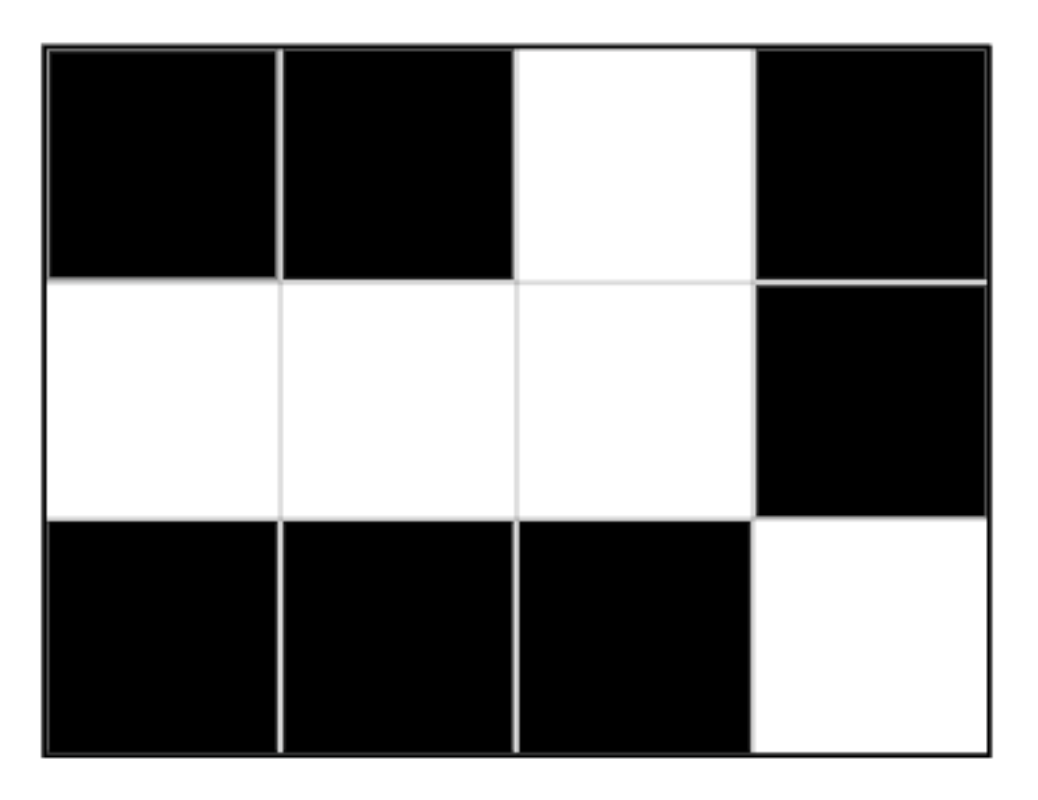
\includegraphics[width=0.2\textwidth, valign=m]{figures/maze.png}
    \end{tabular}
\end{center}

If the starting point is $(1, 2)$, then the nearest exit, located at $(0, 2)$, is one step away. At a high level, this problem asks us to find the shortest path in a matrix, so we should consider breadth-first search which explores cells in order by their distance from the starting point. Every time we explore a cell, we'll check if it's a possible exit, and keep track of its distance from the starting point. If it is, we can terminate the search algorithm and output the distance. A slightly expanded explanation of the algorithm follows:
\begin{enumerate}
    \item Initialize an empty queue to store explored nodes. 
    \item Add the starting point to the queue with distance 0, and mark it as explored. 
    \item While we have not yet reached an exit, and the queue is non-empty, we pop from the queue a vertex $u$ and explore its neighbors (in the four directions specified previously). If the neighbor is an exit, we can terminate the loop and return its distance from the starting location. Otherwise, we mark the neighbor as explored and add it to the queue with its corresponding distance. 
    \item If we fail to find an exit, we return $-1$. 
\end{enumerate}

\IncMargin{2em}
\begin{algorithm}[H]
    \footnotesize
    \DontPrintSemicolon
    \setstretch{1.125}
    \SetKwProg{Fn}{Function}{:}{}
    \SetKwFunction{FindNearestExit}{FindNearestExit}
    \SetKwFunction{len}{len}
    \SetKwFunction{enqueue}{enqueue}
    \SetKwFunction{dequeue}{dequeue}
    \SetKwInOut{Input}{Input}\SetKwInOut{Output}{Output}
    \Input{Matrix $m$, starting point $s = $ (row, column)}
    \Output{Distance of nearest exit; $-1$ if no exit is possible}
    \BlankLine
    \Fn{\FindNearestExit{$m$, $s$}}{
        rows $\gets$ \len{$m$}\; 
        cols $\gets$ \len{$m[0]$}\; 
        
        \BlankLine \BlankLine
        start\_row $\gets$ $s[0]$\;
        start\_col $\gets$ $s[1]$\; 

        \BlankLine \BlankLine
        dirs $\gets$ $[(1, 0), (-1, 0), (0, 1), (0, -1)]$ \; 
        $m$[start\_row][start\_col] $\gets$ `$+$' \; 

        \BlankLine \BlankLine 
        $q \gets$ new queue \; 
        $q$.\enqueue{\upshape[start\_row, start\_col, 0]}

        \BlankLine \BlankLine 
        \While{$q$ \upshape is not empty}{
            $u$ $\gets$ $q$.\dequeue{} \; 
            $u$\_row $\gets$ $u[0]$\; 
            $u$\_col $\gets$ $u[1]$\;
            $u$\_dist $\gets$ $u[2]$ \; 

            \BlankLine \BlankLine 
            \For{\upshape each $d$ \upshape in dirs}{
                next\_row $\gets$ $u$\_row $+ d[0]$\; 
                next\_col $\gets$ $u$\_col $+ d[1]$ \; 

                \BlankLine \BlankLine
                \uIf{\upshape next cell in direction $d$ is a valid unvisited location}{
                    \uIf{\upshape empty cell is a valid exit}{
                        \Return{\upshape $u$\_dist $+ 1$} \; 
                    }
                    \BlankLine \BlankLine
                    $m$[next\_row][next\_col] $\gets$ `$+$' \; 
                    $q$.\enqueue{\upshape[next\_row, next\_col, $u$\_dist $+ 1$]}
                }
            }

        }
        \Return{$-1$}
    }
\end{algorithm}\DecMargin{2em} 

This example illustrates a key difference between graph representations. Although the algorithm relies on BFS, the input ``graph'' is given as an adjacency matrix. Adding to and popping from the queue are $O(1)$ operations; checking the neighbors and marking them as explored also takes $O(1)$. However, in the worst-case, it is possible that the algorithm runs for $O(m \times n)$ nodes before the algorithm terminates. Thus, the runtime is $O(m\times n)$.

\end{document}